\subsubsection{Contexte métier}
\begin{frame}
  \frametitle{Contexte métier}
  \begin{figure}[htbp]
	\centering
	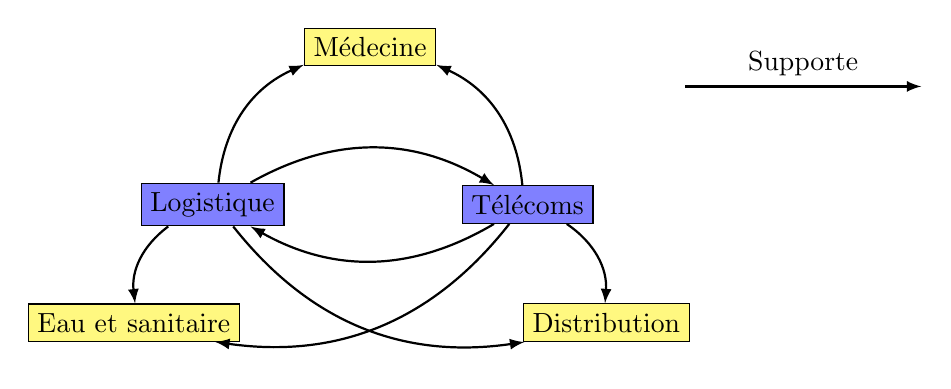
\begin{tikzpicture}
		% définition des styles
		\tikzstyle{metier}=[rectangle,draw,fill=yellow!50,text=black]
		\tikzstyle{support}=[rectangle,draw,fill=blue!50,text=black]
		\tikzstyle{supporte}=[->,>=latex,thick,rounded corners=4pt]
		% les nœuds
		\node[metier] (e) at (-3,-3) {Eau et sanitaire};
		\node[metier] (m) at (0,0.5) {Médecine};
		\node[metier] (d) at (3,-3) {Distribution};
		\node[support] (l) at (-2,-1.5) {Logistique};
		\node[support] (t) at (2,-1.5) {Télécoms};
		% les flèches
		\draw[supporte] (l) to[bend left] (t);
		\draw[supporte] (l) to[bend right] (e);
		\draw[supporte] (l) to[bend left] (m);
		\draw[supporte] (l) to[bend right] (d);
		\draw[supporte] (t) to[bend left] (l);
		\draw[supporte] (t) to[bend left] (e);
		\draw[supporte] (t) to[bend right] (m);
		\draw[supporte] (t) to[bend left] (d);
		% la légende
		\draw[supporte] (4,0) -- (7,0) node[midway,above]{Supporte};
	\end{tikzpicture}
	\caption{Dépendances entre les métiers}
	\label{dep}
\end{figure}
\end{frame}

\begin{frame}
\frametitle{Contexte métier}
\begin{block}
Les processus et les fonctions clefs de la logistique
\end{block}
\begin{block}
Les logisticiens de terrain
\end{block}
\begin{block}
Les transports
\end{block}
\end{frame} 



